\chapter{Oral Presentations}

Nothing should be explained in a way that it cannot be understood by an
intelligent 12 year old.---Albert Einstein

We can all probably remember the anticipation of our first oral
presentation---the sweaty palms, butterflies in the stomach, and the
pressure of trying to remember all the points to be made. Then there is
the fear associated with standing up in front of peers or teachers and
presenting ideas to have them openly criticized. According to a 1973
\ul{London Times} survey, Americans are more afraid of speaking in front
of groups than dying. Perhaps this is due to the fact that although
people know they will die someday, the danger associated with giving a
presentation is more imminent and a greater concern. Somewhere in the
capstone design experience, it is likely that you will have to make an
oral presentation. Examples are the project proposal, a mid-term design
review, and the final presentation. The ability to communicate your
ideas is important beyond your academic career, since practicing
engineers are often required to make oral presentations. Further, your
overall ability to communicate influences how others will accept your
ideas and act upon them---those who communicate clearly are held in high
regard by their peers and tend to advance more quickly. The good news is
that there is help to overcome the fear of oral presentations. With
practice and adherence to some basic principles, one can become a
competent, if not excellent, communicator.

Learning Objectives

By the end of this chapter, the reader should:

\begin{itemize}
\item
  Understand how people evaluate oral presentations.
\item
  Understand common elements of a technical presentation.
\item
  Be able to assemble an effective presentation.
\end{itemize}

\textbf{\hfill\break
DILBERT\textsuperscript{®} by Scott Adams}

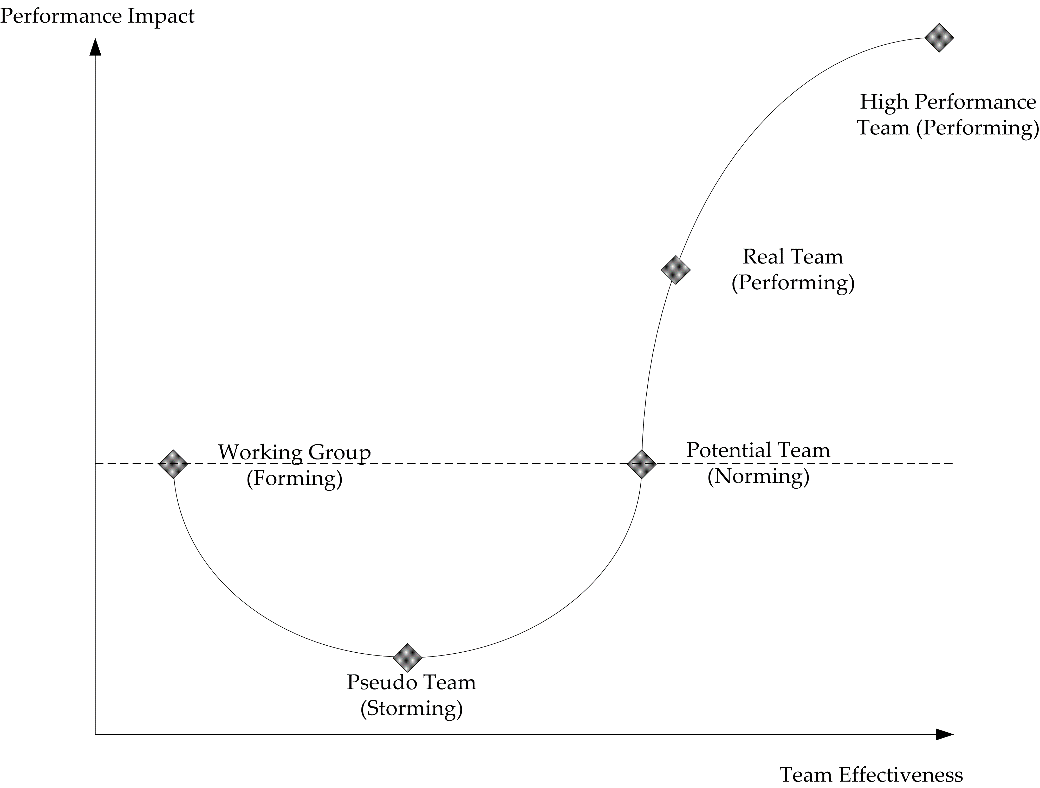
\includegraphics[width=5.5in,height=1.91667in]{Fig/media/image1.png}

\textbf{Figure 12.1} PowerPoint disability. (Dilbert © United Feature
Syndicate. Reprinted by permission.)

\subsection{How People Evaluate
Presentations}\label{how-people-evaluate-presentations}

It is informative to understand how your audience responds to and
evaluates oral presentations. Listening to a presentation is strongly
associated with what is referred to as right-brain activity. Right-brain
activity is dominated by emotion and intuition, while left-brain
activity is associated with logical thinking and reason. This is an
oversimplified model of the brain, but the point is that emotion and
intuition are important elements that people rely on when evaluating a
presentation.

There are three elements, known as the ``three V's,'' that constitute a
presentation: the verbal, the vocal, and the visual. Verbal is what the
speaker says---the actual words and content that come out of the
speaker's mouth. Vocal is indicative of how it is said, and includes
pitch, enthusiasm, inflection, and intonation. Visual is what the
audience sees---the speaker's appearance, eye contact, posture, facial
expressions, and gestures. All three factors go into the evaluation of
speakers, but what is the relative importance of each? The results of a
1964 UCLA study by Dr. Albert Mehrabian (who has bachelors and masters
degrees in engineering and a Ph.D. in psychology) indicates that the
impact of the three elements is 7\% verbal, 38\% vocal, and 55\% visual.
That seems disappointing because we would like to think that the content
of the presentation is most important. Realize that the numbers come
from a simplified study and it is likely that that the percentages would
be different for a highly technical audience. The point is that content
is important, but the other elements can't be ignored. If the visual and
vocal aspects of the presentation are poor, it will be perceived
negatively and make it difficult for the audience to accept and pay
attention to the information presented.

Here is another consideration to think about the next time you make a
presentation or meet somebody. In the first seven seconds of meeting
someone, people typically form a great number of subconscious opinions
about the person they meet {[}Bai81{]}. This includes the person's
income level, education level, competence, character, trustworthiness,
personality, confidence, intelligence, work ethic, and dependability.
Based on what factors are the opinions made? They include appearance,
dress, posture, and speech patterns.

\subsection{Preparing the
Presentation}\label{preparing-the-presentation}

In order to make an effective presentation, the presenter must
understand the subject matter (substance counts), understand the needs
of the audience, and prepare the presentation. The remainder of this
section provides guidance for preparing the presentation.

\subsubsection*{Analyze the Audience}\label{analyze-the-audience}
\addcontentsline{toc}{subsubsection}{Analyze the Audience}

An oral presentation is for the benefit of the audience, not the
presenter. It is necessary to analyze and understand the audience's
needs and prepare the presentation to meet them. For example, a
presentation for engineering professors would likely be different from
one for your family and friends. Analyzing the audience is no different
than the process that one goes through when writing a document. Some
questions to ask in this process are {[}Bai81{]}:

\begin{itemize}
\item
  What are they interested in?
\item
  What do they want from your talk?
\item
  What does the audience already know about my subject?
\item
  What don\textquotesingle t they know?
\item
  What is the attitude of the audience towards me and my subject?
\item
  What are the values of the audience?
\item
  What do you want them to know or learn?
\end{itemize}

Understanding the needs of the audience and putting their interests
first establishes credibility so that they are more willing to accept
the content of the presentation.

Before creating the presentation, identify the main points that the
audience should take away from it. A rule of thumb is to identify three
main points for a talk, as people tend to forget more than that.
Although it is not a strict rule, keep the number of points in that
range, say two to five. Once the points are identified, organize the
presentation to support them.

\subsubsection*{Organize the
Presentation}\label{organize-the-presentation}
\addcontentsline{toc}{subsubsection}{Organize the Presentation}

Just like a story, a presentation has an introduction, a body, and a
conclusion. This is encapsulated in the often-heard wisdom for
presentations to ``tell them what you are going to tell them'' (the
introduction), ``tell it to them'' (the body), and ``tell them what you
just told them'' (the conclusion).

The introduction is absolutely critical---if the audience does not
understand the presentation from the outset, they will tune out.
Einstein's advice that nothing should be explained in such a way that it
cannot be understood by an intelligent 12 year old is particularly
relevant here. Take time to explain the problem in simple terms. Part of
an effective introduction is obtaining the interest of the audience.
There are many ways to accomplish this, and examples include the use of
rhetorical questions or the narration of an experience that the audience
can relate to. This should have to do in some way with the information
being presented. Overall, the objective is to motivate the audience by
describing what is being presented and why it is important. After giving
motivation of the problem, an overview of the talk can be provided. The
overview should be relevant to the problem at hand, not a generic one
that can apply to virtually any presentation.

Structure the body of the presentation to support the main points. This
is done by having a group of two to four related slides that support
each of the main points. The first slide of the group provides some key
ideas, followed by the remaining slides that go into more detail on the
particular point. Don\textquotesingle t make the talk unnecessarily
technical or use a lot of jargon. This does not mean that it should not
have technical content, but that judgment should be exercised in
presenting the right amount of detail. The level of technical detail
depends upon the education and experience of the audience. If it is
necessary to use jargon or acronyms, make sure that they are defined for
the audience. Consider alternative ways of explaining things. The use of
analogies is particularly powerful when explaining complex and abstract
material. One strategy is to increase the level of complexity as the
talk proceeds. That way, much of the early material will be
understandable to the majority of the audience, while the latter more
complex material may only be understood by a small fraction. Everybody
will then leave the presentation with some understanding of the content.

In a typical engineering classroom lecture, the professor usually goes
through many steps in defining and deriving equations. Realize that the
goals of a classroom lecture are very different from that of an oral
presentation. When working with equations, don\textquotesingle t derive
or give too many intermediate steps, unless that is the point of the
presentation. Provide assumptions, selected intermediate equations, and
the important results. Audiences generally assume you have done your
homework and derived the equations properly. There is a tendency to
present equations, vaguely refer to them, and then move on. Equations
should be presented for a reason, so talk about them and describe their
significance. Every equation has its own story; it is the presenter's
job to tell it. The same is also true of graphs and plots.

The conclusion provides the opportunity to summarize and emphasize the
main points of the presentation. Again, tell them what you told them by
reviewing the important points and conclusions. That way if somebody was
lost during the presentation, they can understand the importance of the
work. If there are recommendations to be made for future action, address
them here. The conclusion is also an opportunity to explain the next
steps for the project.

\subsubsection*{Lay Out the Slides}\label{lay-out-the-slides}
\addcontentsline{toc}{subsubsection}{Lay Out the Slides}

Below are pointers for the layout of the slide content.

\begin{itemize}
\item
  \emph{Use a large font}. This ensures that information on the slides
  can easily be seen by the audience. 24 point or greater font is
  typically sufficient.
\item
  \emph{Have a goal of five-to-seven bullet points per page}. Avoid the
  tendency to cram as much information as possible on a page, which is
  often done so that the presenter does not neglect any material. Avoid
  this, and use five to seven bullet points to guide the discussion.
  Presentation software packages, such as Microsoft PowerPoint™, allow
  you to introduce bullet items one at a time, which help to keep the
  discussion on track.
\item
  \emph{Avoid fancy graphics and special effects that add no value}.
  Presentation packages allow the addition of fancy features, such as
  spiraling text and sound effects. They add little to the presentation
  and when overused distract from the content. The content and material
  are what matter the most, not fancy formatting and special effects. To
  quote Edward Tuft, professor emeritus at Yale,

  \emph{Power Corrupts, PowerPoint Corrupts Absolutely.}

  His point is that fancy graphics and features are used far too much
  with PowerPoint presentation software, and that this overpowers both
  the content and the audience. {[}Tuf03{]}.
\item
  \emph{Group slides together to make a major point}. Make the first
  slide the general one with key statements. The following ones should
  have more detailed information supporting the point.
\item
  \emph{Do not create a canned talk or speech}. That is acceptable in
  some fields, but not in engineering and science where a more
  extemporaneous style is the norm. Let the bullet points and other
  material on the slides serve as guides for what to say. Avoid the use
  of cue cards and do not just read directly from the slides for the
  presentation.
\end{itemize}

\subsubsection*{Meet the Time
Constraints}\label{meet-the-time-constraints}
\addcontentsline{toc}{subsubsection}{Meet the Time Constraints}

Make sure that the presentation falls within the time constraints---the
audience will be alienated if it is far too short or too long. The
tendency is to exceed the time limit since there is so much information
that the presenter wants to convey. You may be abruptly cut off and not
be able to conclude the presentation if the time limit is exceeded.
Think about this---how would you describe all that you know about
electrical or computer engineering in ten minutes? It is challenging,
but if you only had ten minutes you would probably give a brief overview
of the major accomplishments made in the field. Accept that all of the
information can't be conveyed in the given time and use it carefully to
highlight the important material.

A heuristic is to take the length of the allotted time in minutes and
divide it by two. That provides an estimate of the number of slides to
prepare. Once the presentation is prepared, practice to see if it can be
presented reasonably in the time allotted. Practice the talk in front of
your teammates, boyfriend, girlfriend, mother, or pet rock. Be careful
not to over-prepare to the point of sounded scripted. Practice the talk
the night before the presentation and only do a brief review of the
material right before the talk. Be sure to allow time for the question
and answer session that usually occurs at the end of a presentation.

\subsubsection*{Prepare for the Question and Answer
Session}\label{prepare-for-the-question-and-answer-session}
\addcontentsline{toc}{subsubsection}{Prepare for the Question and Answer
Session}

One of the biggest fears of presenters is the dreaded question and
answer session. This is where the audience gets to ask questions and
possibly expose the presenter for what they don't know. For example, the
questioner may ask ``\emph{Are you familiar with the work of Johnson and
Smith from 1984 in which they proposed exactly the same idea as yours?"}

How do you prepare for this? You must be knowledgeable about the
subject, but you don't need to have the answers to every possible
question. It is good practice to rephrase questions that are asked for
the benefit of you, the audience, and the questioner. Rephrasing the
question ensures that you are answering the correct question (how many
times have you been annoyed when a teacher answered the wrong question?)
and provides time to think and formulate a response. It demonstrates to
the questioner that you understand their question and are able to
present it in a different format. If the questioner is hostile, make
sure that you rephrase the question in a positive light. Rephrasing is
also a courtesy for the other members of the audience who may have not
heard or understood the question.

Most questions are made in good faith as the questioner is trying to
clarify a point or learn more. Sometimes, questioning can become hostile
or aggressive. If this happens, make sure not to respond in kind or put
the questioner down. The presenter has the position of power and becomes
a bully if they do this. Be sure to maintain eye contact with the
questioner, smile, and remain relaxed in your responses. If you can't
answer the question, admit it and don't try to come up with a phony
answer. If the questioner is persistent, offer to discuss it in more
detail with them after the presentation.

\subsection{Project Application: Design
Presentations}\label{project-application-design-presentations}

Examples of the three presentations that you may make during the design
process are listed in Table 12.1. It is a guide of points to consider
preparing presentations and should be adjusted to meet particular needs
of the situation. The checklist in Table 12.2 is provided to aid in
preparing for presentations.

\textbf{\hfill\break
Table 12.1} Guide for preparing design presentations. The chapters
associated with the points are identified.

\begin{longtable}[]{@{}
  >{\raggedright\arraybackslash}p{(\columnwidth - 2\tabcolsep) * \real{0.1477}}
  >{\raggedright\arraybackslash}p{(\columnwidth - 2\tabcolsep) * \real{0.8523}}@{}}
\toprule\noalign{}
\begin{minipage}[b]{\linewidth}\raggedright
\textbf{Presentation}
\end{minipage} & \begin{minipage}[b]{\linewidth}\raggedright
\textbf{Points to Consider in Preparing the Presentation}
\end{minipage} \\
\midrule\noalign{}
\endhead
\bottomrule\noalign{}
\endlastfoot
Project Proposal & \emph{Introduction.} Provide an overview of the
project and address the need, motivation, goals, and objectives. The
audience is probably not familiar with the concept and it is important
to describe the problem in simple and concise terms (Chapter 2).

\emph{Problem Analysis.} Indicate what the current state-of-the-art in
the field is regarding the technology. If it is a new product concept,
identify similar products that are available and what is unique about
this one. If it is a research-oriented project, include the basic theory
and address current status of work in this area (Chapter 2).

\emph{Requirements Specifications.} Address the engineering requirements
and provide a justification for their selection. Describe the standards
and constraints that apply to the problem (Chapter 3).

\emph{Preliminary Design Options.} Depending upon progress, some
preliminary options for the design may have been developed and can be
presented here (Chapter 4). \\
Design Review & \emph{Introduction.} Provide a brief overview of the
motivation for the project.

\emph{Requirements.} Recap the critical requirements that have to be
met.

\emph{The Proposed Design.} Present the high-level design. Explain how
it works and how the pieces fit together. Include design details of the
sub-components and systems. Address how the proposed design meets the
engineering requirements. Identify the alternatives investigated
(Chapters 4, 5, and 6).

\emph{Preliminary Test Results}. Include test and prototype results
(Chapter 7).

\emph{Project Plan.} By this point (if not earlier), a project plan
should be in place, so consider presenting a summary of the plan
(schedule, responsibilities, and cost) (Chapter 10). \\
Final Presentation & \emph{Introduction.} Provide an overview or
motivation for the project.

\emph{The Final Design.} Describe the final design implementation. A
good way to organize is to provide a high-level overview of the design
and describe how it operates. Then, provide detail and a description for
each of the successive hardware/software subsystems (Chapters 5 and 6).

\emph{Testing \& Results.} Describe/demonstrate the key tests and
results that show the functionality of the design. Provide
demonstrations if appropriate. Indicate how the final realization did or
did not meet the requirements (Chapter 7).

\emph{Conclusions.} Summarize conclusions about the project and provide
recommendations for further work. Indicate lessons learned. \\
\end{longtable}

\textbf{\hfill\break
Table 12.2} Checklist and self-assessment for oral presentation
preparation. Score the elements as 1 = Strongly Disagree, 2 = Disagree,
3 = Neutral, 4= Agree, 5 = Strongly Agree.

\begin{longtable}[]{@{}
  >{\raggedright\arraybackslash}p{(\columnwidth - 2\tabcolsep) * \real{0.8818}}
  >{\raggedright\arraybackslash}p{(\columnwidth - 2\tabcolsep) * \real{0.1182}}@{}}
\toprule\noalign{}
\begin{minipage}[b]{\linewidth}\raggedright
\textbf{Organization}
\end{minipage} & \begin{minipage}[b]{\linewidth}\raggedright
\textbf{Score}
\end{minipage} \\
\midrule\noalign{}
\endhead
\bottomrule\noalign{}
\endlastfoot
The background and needs of the audience were analyzed. & \\
The main points of the presentation are identified. & \\
The motivation is clear and would be understandable to an intelligent 12
year old. & \\
An overview of the presentation is provided. It is relevant to the
presentation, not a generic one that can be used in any presentation.
& \\
The body is organized to support the main points. & \\
The conclusion summarizes the main points and future work. & \\
\textbf{Visual Aids} & \\
The fonts and graphics are large enough to be seen by the audience. & \\
The equations are of the right number and level. The presenters are
prepared to discuss any equations presented. & \\
The slides are arranged to support the main points. & \\
The presentation does not contain unnecessary graphics and special
effects. & \\
\textbf{Presentation Delivery} & \\
The presentation has been rehearsed. It meets the time constraints and
there is sufficient time for questions and answers. & \\
Voice projection is loud enough so that the audience can hear the
presenters. & \\
All members participate in the presentation and have reasonably equal
responsibilities. (If one team member always presents the introduction
and another the technical material, it is a sign that not all members
are participating equally on the project). & \\
The presenters do not rely on cue cards. & \\
The presenters are comfortable in front of an audience (Do they make
good eye contact with the audience? Do the presenters move around the
room or do they stand stiffly behind a podium?) & \\
All presenters are knowledgeable on the subject and prepared to answer
questions. & \\
The presentation software was tested on the platform to make sure it
works. & \\
The presenters are dressed properly for the occasion. & \\
\end{longtable}

\subsection{Summary and Further
Reading}\label{summary-and-further-reading}

During the design process and your professional career, you will need to
communicate ideas effectively. One of the most common ways to do this is
via an oral presentation. Visual, verbal, and vocal aspects impact the
effectiveness of an oral presentation. Although the verbal aspect, or
content, is important, the visual and vocal delivery aspects heavily
influence the audience's perception and cannot be overlooked. In
preparing the presentation, the needs and background of the audience
should be taken into consideration and the main points to be conveyed
identified. Creating the presentation is much like telling a
story---there should be an introduction, a body, and a conclusion that
are organized to support the main points. The slides should be grouped
to support these points. Concepts should be explained as simply and
clearly as possible. Increasing the complexity as the presentation
proceeds will allow the presentation to reach all members of the
audience to some extent. Practicing the presentation is especially
important for novice presenters, and tips were provided for meeting the
time constraints and preparing for question sessions.

There are many excellent resources and articles available regarding oral
presentations. A concise and humorous article geared for new speakers in
the technical fields is \emph{Advice to Beginning Physics Speakers} by
James Garland {[}Gar91{]}. The \ul{IEEE Transactions on Professional
Communications} journal addresses many aspects of communications
including oral presentations. Mindtools
(\href{http://www.mindtools.com}{www.mindtools.com}) has a section on
communication skills that includes a preparation checklist on
presentation, delivery, appearance, and visual aids. \emph{A Good Speech
is Worth a Thousand Words} by Bert Decker {[}Dec84{]} addresses right
and left brain thinking as well as the three V's of giving a
presentation. The article \emph{How to Overcome Errors in Public
Speaking} by John Baird {[}Bai81{]} addresses how to analyze the
audience, the judgments that are made when meeting a person, the
introduction, and conclusion. Other resources used in the preparation of
this chapter include: \emph{The Engineering Presentation---Some Ideas on
How to Approach and Present It} {[}Ros93{]}, \emph{Handling a Hostile
Audience---With Your Eyes} {[}Car89{]}, and \emph{How to Speak so that
Facts Come Alive} {[}Ste89{]}. Many of the references are compiled in
the book \ul{Writing and Speaking in the Technology Professions: A
Practical Guide} edited by David Beer {[}Bee03{]}.
